\definecolor{rouge_inria}{RGB}{180,0,0}

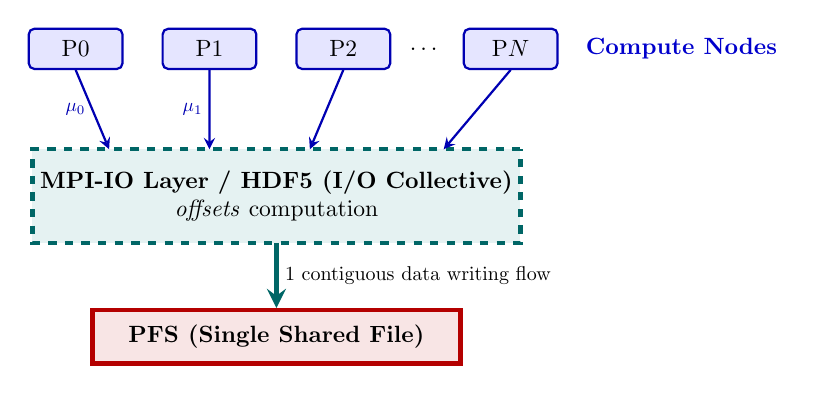
\begin{tikzpicture}[
    scale=0.85, every node/.style={transform shape},
% Block styles
    mpi/.style={rectangle, draw=blue!70!black, fill=blue!10, thick, minimum width=1.4cm, minimum height=0.6cm, rounded corners=2pt},
    agg/.style={rectangle, draw=teal!80!black, fill=teal!10, dashed, ultra thick, minimum width=6.5cm, minimum height=1.4cm, align=center},
    pfs/.style={rectangle, draw=rouge_inria, fill=rouge_inria!10, ultra thick, minimum width=5.5cm, minimum height=0.8cm, align=center}
]

% 1. Processes (data scattered in memory)
\node[mpi] (mpi0) at (-3, 2.5) {P0};
\node[mpi] (mpi1) at (-1, 2.5) {P1};
\node[mpi] (mpi2) at (1, 2.5) {P2};
\node (mpidots) at (2.2, 2.5) {$\dots$};
\node[mpi] (mpiN) at (3.5, 2.5) {P$N$};
\node[anchor=west, text=blue!80!black] at (4.5, 2.5) {\textbf{Compute Nodes}};

% 2. Aggregation step (collective I/O)
\node[agg] (aggregation) at (0, 0.3) {\textbf{MPI-IO Layer / HDF5 (I/O Collective)}\\ \textit{offsets} computation};

% Arrows processes -> aggregation
\draw[->, >=stealth, thick, blue!70!black] (mpi0.south) -- (-2.5, 1) node[midway, left, scale=0.8] {$\mu_0$};
\draw[->, >=stealth, thick, blue!70!black] (mpi1.south) -- (-1, 1) node[midway, left, scale=0.8] {$\mu_1$};
\draw[->, >=stealth, thick, blue!70!black] (mpi2.south) -- (0.5, 1);
\draw[->, >=stealth, thick, blue!70!black] (mpiN.south) -- (2.5, 1);

% 3. Single write to the PFS
\node[pfs] (pfsfile) at (0, -1.8) {\textbf{PFS (Single Shared File)}};

% Single contiguous write flow
\draw[->, >=stealth, line width=2pt, teal!80!black] (0, -0.4) -- (pfsfile.north) 
        node[midway, right, text=black, scale=0.85] {1 contiguous data writing flow};

\end{tikzpicture}